\documentclass[,table]{beamer}

% Modèle proposé par Aurélie Boisbunon

% ATTENTION : IL FAUT EXECUTER LE CODE 2 FOIS POUR QUE LES IMAGES
% SOIENT AU BON ENDROIT

% Theme du poster
\usetheme{posterLITIS2}
%\usetheme{posterLITIS}

% Mise en page poster
\usepackage[orientation=portrait,size=a1 ,scale=1.2]{beamerposter} 

\usepackage[english]{babel}
\usepackage[utf8]{inputenc}
\usepackage{times} % Police du texte
\usepackage{amsmath,amsthm, amssymb, latexsym} % Packages pour
% formules maths
\usepackage{dsfont} % Package pour l'indicatrice

% Package et librairies pour dessins et figures : package 
\usepackage{pgf,tikz} 
\usetikzlibrary{calc,trees,positioning,arrows,chains,shapes.geometric,%
  decorations.pathreplacing,decorations.pathmorphing,shapes,%
  matrix,shapes.symbols,shapes.arrows}

% Pour surligner la ligne des tableaux
\definecolor{Mygrey}{gray}{0.8} 

% Couleur des sous-titres dans les cadres et du texte en vert
\newcommand{\soustitre}[1]{\vspace{5pt}{\small\textbf{\textcolor{bleuL}{#1}}}} % 
\newcommand{\exemple}[1]{\textcolor{vertL!92!black}{#1}} % 

% Si on veut une image de fond
% \setbeamertemplate{background canvas} 
% { 
% \begin{tikzpicture}
%   \node[inner sep=0pt,xshift=20cm]  at (current page.center)
%   {
\includegraphics[width=.5\paperwidth]{LITIS_fond.png}};
% \end{tikzpicture} 
% } 

%   ******************************************************************************************
%   Definition des elements du graphe tikz
\tikzset{
  >=stealth',
  punktchain/.style={
    ellipse, 
    draw=rougeF!80, thick,
    top color=red!10,              % a shading that is white at the top...
    bottom color=rougeF!70,
    text width=4.3em, 
    minimum height=2em, 
    text centered, 
    on chain},
  line/.style={draw, ultra thick, <-},
  every join/.style={->, ultra thick ,shorten <=2pt,
    shorten >=2pt,},
}

% *******************************************************************************************
% EN-TETE ET PIED DE PAGE
% *******************************************************************************************

% Chemin pour repertoire d'images
\graphicspath{{imgs/}}

% Titre, auteurs, institut, date
\title{Criteria \ for \ Variable \ Selection \ with \ Dependence}
\author[Boisbunon et al.]{Aurélie Boisbunon, Stéphane Canu, Dominique Fourdrinier}
\institute[LITIS]{Université de Rouen and INSA de Rouen}
% \date{Dec. 16th, 2011}

% Logos 
\newcommand{\logolitis}{logo_litis_bleu_transp.png}
\newcommand{\logoinstitut}{logo-univ-rouen.png}
\newcommand{\logolaboratoire}{logo_insa.png}

% Pied de page avec adresse site Litis et adresses mail des auteurs
\newcommand{\foottextleft}{http://www.litislab.eu} % texte a gauche
\newcommand{\foottextright}{ \{firstname.name\} @ litislab.fr  } % texte a droite

% *******************************************************************************************
% CONTENT
% *******************************************************************************************

\begin{document}
\begin{frame}{} 
  \begin{columns}
    \begin{column}{0.70\linewidth}
      \begin{block}{Abstract}
        \begin{itemize} 
        \item Derivation of a new criterion through \exemple{loss
            estimation}
        \item Valid under the \alert{spherical} assumption allowing
          for \alert{dependence} between observations
        \item Integration in a whole procedure from model
          exploration to model evaluation
        \end{itemize}
      \end{block}
    \end{column}
  \end{columns}

  % *****************************************************************************************

% UN GROS CADRE AVEC DEUX COLONNES A L'INTERIEUR
  \vfill
  \begin{columns}
    \begin{column}{.915\paperwidth}
      \begin{block}{Context}
        \begin{columns}[t]
          \begin{column}{.45\linewidth}
            \soustitre{Linear regression model}
            \begin{displaymath}
              Y = X\beta + \varepsilon \quad \left\{
                \begin{array}{l}
                  Y \in\mathbb{R}^n\\ X
                  \in\mathbb{R}^n\times\mathbb{R}^p \text{
                    (fixed)}\\ \beta \in \mathbb{R}^p \\
                  \varepsilon \in \mathbb{R}^n \alert{\sim \mathcal{S}_n(0)}
                \end{array}
              \right.
            \end{displaymath}
            \begin{itemize}
            \item Aim: sparse estimation of $\beta$
            \end{itemize}
          \end{column}
          \begin{column}{.45\linewidth}
            \vspace{-15pt}
            \begin{itemize}
            \item Literature based exclusively on either
            \end{itemize}
            \begin{list}{-}{\leftmargin=2em}
            \item estimation of a sparse $\beta$
            \item evaluation of several models
            \end{list}

            \vspace{10pt}
            \begin{itemize}
            \item Mostly rely on independence 
            \end{itemize}
            \begin{list}{-}{\leftmargin=2em}
            \item generally not true in real examples
            \end{list}
          \end{column}
        \end{columns}
      \end{block}
    \end{column}
  \end{columns}

  % *****************************************************************************************

% DEUX PETITS CADRES SEPARES SUR DEUX COLONNES
  \vfill

  \begin{columns}[t]
    \begin{column}{.45\linewidth}
      \begin{block}{Framework}
        \soustitre{Spherically symmetric distributions $\mathcal{S}_n$}
        \begin{itemize}
        \item No need to specify the form of the distribution
        \item \alert{Dependence} between the components of $Y$
        \item Distributional robustness
        \end{itemize}

        \begin{figure}[h]
          \centering
          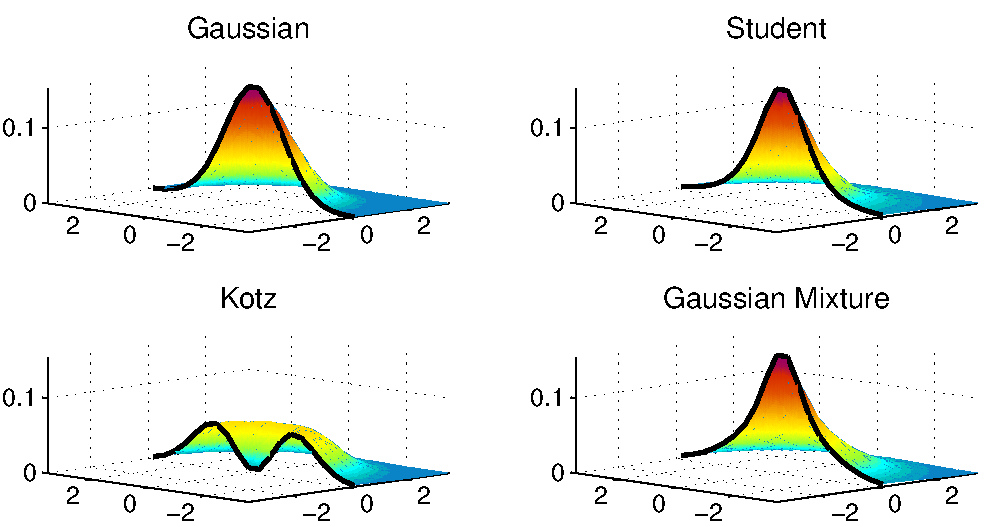
\includegraphics[width =\linewidth]{lois_SS_3D}
        \end{figure}

        \soustitre{Model Selection steps}
        \vspace{15pt}
        \begin{center}
          \begin{tikzpicture}
            [node distance=1cm,  auto,start chain=going below right,]
            \node[punktchain] (explor) [label= right:{\small\textit{e.g.}
              $\displaystyle{\max_{j\le p}}\,\bold{x}_j^t(y-X\hat\beta)$}] {Exploration};% 
            \node[punktchain] (estim) [label=below left:{\small\textit{e.g.} $\hat\beta^{LS}$}]{Estimation};
            \node[punktchain] (eval) [label=below left:{\small\textit{e.g.} AIC/$C_p$}]{Evaluation};
            \path[->, ultra thick] (explor) edge [bend right=45] (estim);
            \path[->, ultra thick] (estim) edge [bend right=45] (eval);
          \end{tikzpicture}
        \end{center}
      \end{block}
    \end{column}  

    % ****************************************************************************************

    \begin{column}{.45\linewidth}
      \begin{block}{Procedure}
        \soustitre{Firm Shrinkage / MC+}
        \begin{itemize}
        \item Exploration: \exemple{regularization path} 
        \item Estimation: \exemple{nearly unbiased} estimator
        \end{itemize}
        \begin{displaymath}
          \hat\beta^{FS}_j(\lambda) = \left\{
            \begin{array}{l l}
              0 & |\hat\beta^{LS}_j|\le \lambda \\
              \alpha(\hat\beta^{LS}_j-\lambda sign(\hat\beta^{LS}_j))/(\alpha-1) & \lambda<|\hat\beta^{LS}_j|\le \alpha\lambda \\
              \hat\beta^{LS}_j & |\hat\beta^{LS}_j|> \alpha\lambda
            \end{array}
          \right.
        \end{displaymath}
        {\small
          \begin{itemize}
          \item $\lambda>0 \, \rightarrow$ tunes sparsity, $\alpha>1 \, \rightarrow$ tunes bias
            \vspace{5pt}
          \item $\hat\beta^{LS}= (X^tX)^{-1}X^ty\;$ (least-squares estimator)
          \end{itemize}
        }      \vspace{40pt}

        \soustitre{Evaluation: Loss estimation}
        \begin{itemize}
        \item \exemple{Loss function}
          $L(\hat\beta,\beta)=\|\underbrace{X\hat\beta}_\text{estimate}-\underbrace{X\beta}_\text{true}\|^2$
        \item Estimation $\widehat{L}$ of $L$
          \vspace{5pt}
          \begin{itemize}
          \item Step 1: unbiased estimator $\widehat{L}_0 \setminus \forall
            \beta \;
            \mathbb{E}_Y[\widehat{L}_0]= \mathbb{E}_Y[L(\hat\beta,\beta)]$% 
            \vspace{5pt}
          \item Step 2: improvement $\widehat{L}_\rho \setminus \mathbb{E}_{Y}(\widehat{L}_\rho-L)^2
            \le \mathbb{E}_{Y}(\widehat{L}_0-L)^2$
          \end{itemize}
        \end{itemize}
        \vspace{15pt}
        \begin{center}
          \tikz[baseline]{
            \node[fill=red!15,anchor=base] (t2)
            {$\widehat{L}_\rho =
              \|y-X\hat\beta^{FS}(\lambda)\|^2+(2df-n)\frac{\|y-X\hat\beta^{LS}\|^2} {n-p}
              \,\alert{ \boldsymbol{-\rho(y)} }$};
          } 
        \end{center}
        {      \small
          \begin{list}{$\hookrightarrow$}{\leftmargin=2.7em}
          \item Correction function: $\rho(y) =C \gamma^{-1}(y) \|y-X\hat\beta^{LS}\|^4 $
            \vspace{3pt}
          \item $\gamma(y)=k\max_{i\le
              p}\{(q_i^ty)^2\setminus |q_i^ty|\le\lambda \}+ \sum_{j\le p} (q_j^ty)^2\mathds{1}_{\{ |q_j^ty|\le\lambda \}} $
          \end{list}
        }
        \vspace{15pt}
        \begin{itemize}
        \item Selection: $\hat\lambda = \displaystyle{\arg\min_{\lambda\in\mathbb{R}_+} }\;\widehat{L}_\rho \left(y,\lambda\right)$
        \end{itemize}
        \vspace{7pt}
      \end{block}
    \end{column}  
  \end{columns}

  % *******************************************************************************************

  \vfill
  \begin{columns}
    \begin{column}{.945\linewidth}
      \begin{exampleblock}{Results}
        Example: $ n=40 \text{ observations, } \; p=5 \text{ variables, }
        \; \beta=(2,0,0,4,0)^t, \; r=5000 $ replicates
        \begin{columns}
          \begin{column}{.5\linewidth}
            \begin{displaymath}
              \varepsilon \sim \mathcal{N}_n(0,I_n) 
            \end{displaymath}
            \begin{table}[h]
              \label{tab:firm_gauss}
              \footnotesize
              \begin{tabular}{c *{3}{r@{.}l} r@{.}l@{}r@{.}l | r@{.}l}
                \textbf{Subset}&\multicolumn{2}{c}{$\boldsymbol{\widehat{L}_\rho}$}&\multicolumn{2}{c}{\textbf{AIC}}&\multicolumn{2}{c}{\textbf{BIC}}&\multicolumn{4}{c}{\textbf{LOOCV}}&\multicolumn{2}{c}{\textbf{Real
                    loss}}\\ [3pt]
                \{4\}&26&12 (0.56)&20&18 (0.59)&40&05 (0.83)&14&42&(16&18)&14&17 (0.43)\\
                \makebox[0pt][l]{\fboxsep0pt\colorbox{Mygrey}{\strut\hspace*{.9\linewidth}}}
                \{1,4\}&\textbf{44}&\textbf{41 (0.60)}&39&02 (0.74)&39&37 (0.49)&32&71&(12&27)&54&29 (0.56)\\
                \{1,2,4\}& 1&33 (0.15)& 7&57 (0.34)& 3&66 (0.26)& 5&68&(3&06)& 7&46 (0.33)\\
                \{1,3,4\}& 1&30 (0.13)& 7&83 (0.40)& 3&73 (0.19)& 6&93&(2&99)& 7&63 (0.32)\\
                \{1,4,5\}& 2&13 (0.20)& 7&73 (0.40)& 3&73 (0.36)& 6&49&(3&73)& 7&87 (0.27)\\
              \end{tabular}
              \caption{Percentage of selection with Firm
                Shrinkage }
            \end{table}
          \end{column}
          
          \begin{column}{.5\linewidth}
            \begin{displaymath}
              \varepsilon \sim\mathcal{T}_n(\nu=4)
            \end{displaymath}
            \begin{table}[h]
              \footnotesize
              \begin{tabular}{c *{3}{r@{.}l} r@{.}l@{}r@{.}l | r@{.}l}
                \textbf{Subset}&\multicolumn{2}{c}{$\boldsymbol{\widehat{L}_\rho}$}&\multicolumn{2}{c}{\textbf{AIC}}&\multicolumn{2}{c}{\textbf{BIC}}&\multicolumn{4}{c}{\textbf{LOOCV}}&\multicolumn{2}{c}{\textbf{Real
                    loss}}\\[3pt]
                $\emptyset$& 8&87 (0.43)& 9&94 (0.65)&20&90 (0.74)& 7&21&(3&12)&14&62 (0.45)\\
                \{4\}&19&11 (0.29)&15&77 (0.37)&24&33 (0.45)&12&63&(8&99)&14&88 (0.50)\\
                \makebox[0pt][l]{\fboxsep0pt\colorbox{Mygrey}{\strut\hspace*{.9\linewidth}}}
                \{1,4\}&\textbf{38}&\textbf{01 (0.62)}&32&08
                (0.74)&35 &15 (0.82) &26 & 35&(11&77)&46 &08 (0.78)\\
                \{1,2,4\}& 0&00 (0.14)& 6&08 (0.21)& 2&74 (0.16)& 5&82&(2&93)& 4&65 (0.21)\\
                \{1,4,5\}& 1&63 (0.22)& 6&21 (0.36)& 2&83 (0.20)& 6&58&(3&39)& 4&50 (0.16)\\
              \end{tabular}
              \caption{Percentage of selection with Firm
                Shrinkage}
              \label{tab:firm_stud}
            \end{table}

          \end{column}
        \end{columns}
      \end{exampleblock}
    \end{column}

  \end{columns}

  % *******************************************************************************************

  \vfill
  \section{Conclusion}
  \begin{columns}
    \begin{column}{.45\linewidth}
      \begin{block}{Conclusion}
	\begin{itemize}
        \item STOP using AIC, BIC, and LOOCV
        \item USE $\hat{L}_\rho$ instead
        \item Possible application to classification, clustering, etc.
        \end{itemize}
        \vspace{5pt}
      \end{block}
    \end{column}   
    

% BIBLIO
    \begin{column}{.45\linewidth}
      \textbf{References}
      {\footnotesize
        \bibliography{biblio_poster}
        \bibliographystyle{nar}
      }
    \end{column}
  \end{columns}

\end{frame}
\end{document}



%%%%%%%%%%%%%%%%%%%%%%%%%%%%%%%%%%%%%%%%%%%%%%%%%%%%%%%%%%%%%% 

%%% Local Variables: 
%%% mode: latex
%%% TeX-PDF-mode: t
%%% End:
